\part{Desenvolvimento}

\chapter[Comércio]{Comércio}
\section{Considerações iniciais}

O termo comércio deriva do conceito latim \textit{comercium} e refere-se à negociação que tem lugar na hora de comprar ou vender serviços ou mercadorias. Também pode-se chamar de comércio qualquer loja, armazém, estabelecimento ou plataforma digital que realize transações de algo em troca de outra coisa de igual valor, podendo ou não ser dinheiro. Estruturou-se como uma atividade socio-econômica que consiste na compra e venda de bens, serviços ou produtos\footnote{\url{conceito.de/comercio}}. Atualmente existem várias classes de comércio, neste documento será abordado o \textit{E-Commerce}, também conhecido como comércio eletrônico.

\section{Modelos de comércio}

O comércio atual é dividido em duas principais categorias, o comércio físico e o comércio eletrônico, para vias de pesquisa, vamos tratar do comércio eletrônico, aquele em que uma transação pode ser iniciada e finalizada por meio de uma plataforma ou aplicação que tenha conexão a \textit{Web}\footnote{\url{http://www.scielo.br/pdf/rae/v42n3/v42n3a10}}.

\subsection{Comércio eletrônico}

Nesta seção vamos tratar a questão do comércio eletrônico atual, que já é uma realidade nos mais diversos setores da economia, tanto falando de Brasil, como também fora dele. Várias organizações tem o \textit{E-Commerce} como parte de sua estratégia, outras já funcionam exclusivamente a partir do comércio eletrônico. Segundo \cite{rae:2002} tanto no mundo como no Brasil, o comércio eletrônico se encontra em processo de consolidação e a tendência é de crescimento. As realização que estão sendo empreendidas tem como foco principal desenvolver os processos que já existem e criar uma base para que ambientes mais novos possam ser sustentados. A partir de um início simples de fornecimento de informação, percebeu-se o potencial de mercado, sendo asim, buscou-se primeiro a realização de transações, em segundo, formas de apoiar à distribuição, e por ultimo a iteração pela comunicação e pela troca de informações\cite{rae:2002}.

\section{Métodos e Tecnologias}

Será abordado neste tópico as metodologias aplicadas no conceito de comércio eletrônico, a pesquisa no mercado brasileiro fornece subsídios suficientes para confirmar que as empresas estão adequando-se aos novos ambientes, melhorando os processos já existentes e utilizando novas tecnologias já usadas no mercado, principalmente \textit{cookies}, esta situação demostra que as empresas estão se movimentando para que possam evoluir junto a esse tipo de comércio\footnote{\url{http://www.dataversity.net/semantic-commerce-structuring-your-retail-website-for-the-next-generation-web-2/}}

\section{Considerações preliminares}

O comércio acompanha a evolução da sociedade, tendo carater de grande importância no quesito sócio-econômico de países, o comércio interno é aquele que se realiza dentro de um mesmo país, que respondem a uma mesma jurisdição, já o externo diz respeito a transações entre diferentes países. É perceptível um grande crescimento do valor do comércio eletrônico para empresas, por isso esse aumento exponencial da busca por plataformas e tecnologias para aplicar \textit{E-Commerce}.

\chapter{Web semântica e Ontologias}
\section{Considerações iniciais}

Neste capítulo tem-se por objetivo revisar bibliográficamente e introduzir conceitos de \textit{Web Semântica}. Abordando os conceitos, tecnologias e algumas aplicações, assim como levantar o uso de \textit{Web Semântica} em exemplos práticos aplicados a \textit{E-Commerce}.

\section{Web Semântica e Ontologias}

Hoje, com o exponente avanço das tecnologias, que geram mudanças de paradigmas e a maneira com que nos relacionamos e comunicamos, o modo como geramos e recebemos informações caminha junto a esta evolução. A chamada "era da informação" ou "era do conhecimento", as informações geradas e consumidas são vistas como matéria-prima para
 desenvolvimento sócio-cultural e econômico\cite{takahashi:2000}.

A principal destas tecnologias criadas para disseminação de informação é a intenet, através da \textit{World Wide Web} (WWW), considerada a maior fonte de informações concentradas\cite{alves:2004}. Em contrapartida a essa excessiva criação de conteúdo, existe também uma crescente quantidade de informações que são disponibilizadas na rede, gerando problemas de busca e recuperação de conteúdo, por conta de uma falta de organização, mesmo com fortes ferramentas de busca\cite{breitman:2006}

A respeito de busca e recuperação de informações a forma que são disponibilizadas na \textit{web} é utilizando linguagens de marcação, tais quais HTML e XML, onde são configuradas suas propriedades\cite{breitman:2006}. Desta maneira, as funcionalidades de busca realizam sua trabalho por meio de similaridades sintáticas, ou seja, algoritmos que buscam palavras-chave, o que por várias vezes resultam em resultados ineficiêntes ou indesejados, isso por uma palavra ter o poder de assumir diferentes significados, dependendo do contexto a qual está inserida\cite{breitman:2006}.

Sendo assim, em meio a esse "caos" de informações, não existe estratégia que abrange a indexação dos documentos contidos na mesma de maneira satisfatória, recuperar estas informações, por meio de motores de busca, baseia-se prioritáriamente em palavras-chaves contidas no texto dos documentos\cite{souza:2004}

Deste modo, as informações disponibilizadas nada mais são que palavras encontradas em um texto, os computadores tratam de apresenta-las, porém, sem avaliar, classificar ou selecionar essas informações, responsabilidades estas que ficam a cargo dos seres humanos interessados para definir quais informações são condizentes e relevantes a sua busca\cite{breitman:2006}.

Segundo Souza(2006) por mais que a \textit{web} tenha sido, em seu conceito, projetada com a ideia de possibilitar o fácil acesso e agilizar troca de informações, sua implementação ocorreu de forma descentralizada, crescendo exponencialmente e hoje atua como um imenso repositório de documentos, o que deixa a desejar ao que se trata de conceitos relevantes ao conteúdo.

No contraponto ao que é conhecido como \textit{Web Sintática}\cite{berners:2001} a proposta é um mecanismo que capture o significado das palavras de maneira semântica, de forma que os computadores possam processar e relacionar informações capturadas em diferentes fontes e contextos. Baseado nisso, foi proposto a inserção de semântica na estrutura dos documentos disponibilizados via \textit{web}\cite{breitman:2006}. Esta nova arquitetura foi denominada \textit{Web Semântica}, ideia creditada a Tim Berners-Lee e conduzida posteriormente pela W3C, onde o objetivo é acoplar contexto e inteligência na \textit{web} atual, possibilitando melhor uso e recuperação de informações relevantes\cite{souza:2004}.

\begin{quote}
A \textit{Web Semântica} não é uma web separada, mas uma extensão da \textit{web} atual na qual as informações apresentam significados bem definidos e permite que computadores e pessoas possam trabalhar em cooperação\cite{berners:2001}.
\end{quote}

Desta forma, computadores deixam de ser apenas apresentadores de conteúdo e se tornam agentes inteligentes, com a capacidade de entender o significado das informações, e assim, recuperar e manipular de maneira lógica os dados. Para isso, é necessário que na implementação e estruturação de conteúdo, os provedores das páginas \textit{web} organizem suas informações seguindo regras de inferência, possibilitando gerir um raciocínio automatizado\cite{berners:2001}. Esta interligação de informações estruturadas, definidas semanticamente proporcionam uma recuperação de informação mais eficaz, formando uma rede conectada por meio de ferramentas tecnológicas\cite{alves:2004}.

\begin{quote}
A \textit{Web Semântica} é uma rede de informações interligadas de tal modo que possa ser facilemtne processada por máquinas, em escala global\cite{palmer:2009}.
\end{quote}

A \textit{Web Semântica} é composta por três elementos, sendo eles:
\begin{enumerate}
\item Representação do conhecimento - Gera uma estrutura ao conteúdo significativo de páginas \textit{web} criando um ambiente onde agentes inteligente buscam de uma página a outra, podendo executar taréfas mais sofisticadas para usuários;
\item Ontologias -  Considerada a espinha dorsal da \textit{Web Semântica} define um aspecto semântico para representar seres, entes, qualquer que possa ser conveniente se chamar de assunto, conteúdos temáticos dos registros da realidade;
\item Agentes - Tem a função de coletar conteúdo e informações na \textit{web} em diversas fontes, processar e trocar dados entre outros programas, páginas ou aplicações através de linguagem que expressa inferências lógicas, resultado do uso das regras e informações como aquelas especificadas pela ontologia. Assim a máquina passa a reconhecer provas escritas na linguagem, estas quais os programas-agente, através da lógica descrita na ontologia, retorna dados requisitados pela pesquisa, respeitando o contexto.
\end{enumerate}

\subsection{Ontologias}

\begin{quote}
"Ontologia é uma especificação formal e explícita de uma conceitualização compartilhada\cite{gruber:1993}."
\end{quote}

Sendo assim:

\textbf{Especificação Explícita -} Elementos e restrições estão explicitamente conceituados.
\textbf{Especificação Formal -} Agentes portadores de inteligência serão responsáveis pelo processamento automático das informações, dispensando intervenção humana.
\textbf{Conceitualização -} Representação de um modelo abstrato de eventos que identificam os principais conceitos.
\textbf{Compartilhada -} Ontologia capaz de reconhecer um conhecimento consensual, compartilhado por um conjunto de pessoas.

Na computação, ontologia é a documentação ou arquivo utilizado entre as relações entre termos e conceitos, disponibilizando um vocabulário para a comunicação entre agentes e páginas \textit{web}, definindo as relações entres os mesmos\cite{pickler:2007}

Para a W3C\footnote{\url{www.w3c.br}}, a descrição de ontologia é dada pela definição dos termos utilizados na descrição e na representação de uma área de conhecimento. Sendo assim, devem conter obrigatóriamente:
\begin{itemize}
\item Classes - Descrevem conceitos e providenciam uma representação lógica.
\item Propriedades - Caracterizam as propriedades das entidades.
\item Relações - Definem as ligações entre classes e propriedades.
\end{itemize}

A partir dessas definições, o uso de metadados descreve as informações sobre os objetos ou indivíduos\cite{breitman:2006}, onde temos a ideia de dados sobre dados para se referir a qualquer informação utilizada para identificar, descrever ou localizar recursos\footnote.

\subsection{Metadados}

Metadados são as formas de organizar conhecimento, são capazes de dizer do que se trata determinados dados. Através deles computadores são capazes de compreender os assuntos que são tratados. A função dos metadados é facilitar a compreensão dos relacionamentos e a utilidade das informações.

Metadados são definidos pela \textit{International Federation of Library Associations} (IFLA) seguindo esta definição:
\begin{quote}"Metadados são dados sobre dados. O termo se refere a qualquer informação utilizada para identificar, descrever e localizar recursos."\end{quote} e a W3C os define como sendo \begin{quote}"Informações para web que podem ser entendidas por máquinas"\cite{breitman:2006}.\end{quote}

Através das citações acima, percebemos que não existe uma definição única para o tema, o conceito de metadados é antigo, mas ainda é largamente discutido em várias comunidades. Pode ser usado em diversos contextos, não se restringindo a \textit{Web Semântica}. W3C padronizou uma linguaguem para que seja possível aplicar o máximo de semântica possível das ontologias, esta linguagem é a \textit{Resource Description Framework} (RDF).

\subsection{Resource Description Framework}
A linguagem RDF disponibiliza uma \textit{framework} para representar informações, ou metadados, sobre recursos. As principais especificações do RDF contemplam um modelo de dados capaz de fornecer dados sobre dados, sintaxe esta que se baseia em \textit{Extensible Markup Language} (XML) e uma linguagem de definição de esquemas para vocabulários. A ideia de utilizar RDF é alcançar um modelo de dados que possa ser expresso de maneira simples em suas declarações sobre recursos. Cada declaração é formada por sujeito, predicado e objeto\cite{breitman:2006}.

\subsection{Extensible Markup Language}
Aqui falaremos de XML, a tradução literal é "Linguagem de Marcação Extensível", utilizada para organizar hierarquias de dados em documentos, seu aspecto extensível é notado quando se permite definir elementos de marcação, dotado de uma sintaxe básica que pode ser utilizada para compartilhar informações entre diferentes computadores ou aplicações\cite{breitman:2006} como na figura \ref{fig01}.

\begin{figure}[h]
	\centering
	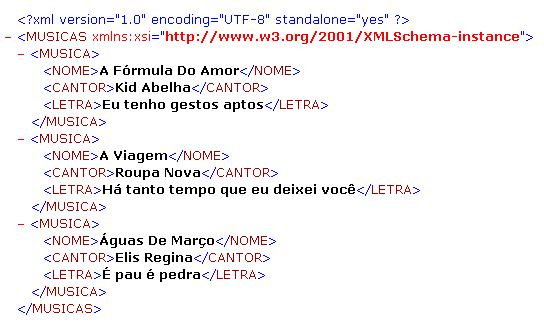
\includegraphics[keepaspectratio=true,scale=1.0]{figuras/exemploXML.jpg}
	\caption{Documento XML para definir músicas. Fonte http://www.tomasvasquez.com.br}
	\label{fig01}
\end{figure}

\subsection{URI - Uniform Resource Identifier}

Nesta arquitetura, além de outros conceitos importantes, temos o uso de um URI (Identificador Uniforme de Recursos) que é responsável por endereçar arquivos e/ou informações pela \textit{web}. Utiliza-se URI como um padrão para identificar um recurso físico ou abstrato de maneira global, mas mantendo sua forma única. Pela W3C\footnote{\url{www.w3c.br}} um URI é definido por uma cadeia de caracteres compacta, usada para identificar ou denominar um recurso por meio da internet. Essa identificação permite a interação com representantes do recurso através de um rede, geralmente sendo a rede mundial de computadores, através de protocolos\cite{alves:2004}.

Um URI pode ser classificado como um localizador, como um nome ou ainda assumir a identidade de ambos. O URN define a identidade de um item, enquanto o URL é responsável por um método que possa encontrar esse item\cite{breitman:2006}.

\subsection{OWL - Web Ontology Language}

A \textit{Web Ontology Language}, lançada pela W3C\footnote, sendo projetada para atender as aplicações \textit{Web Semanticas}, onde podemos citar a construção de ontologias, explicitar fatos sobre um domínio,Racionalizar ontologias e fatos, a linguagem OWL é formada por elementos básicos\cite{breitman:2006}:

\begin{itemize}
	\item Namespaces - Para criar um conjunto de conceitos, é necessário indicar quais vocabulários estão sendo utilizados. As declarações de \textit{namespaces} são feitas entre etiquetas do tipo rdf:RDF permitindo que sejam interpretados sem ambiguidades.
	\item Cabeçalhos - Após a definição de \textit{namespaces} definidos, insere-se uma coleção de sentenças sobre a ontologia, por meio do uso da etiqueta owl:Ontology. Etiquetas estas que registram comentários conceitos informações de outras ontologias e controle de versões.
	\item Classes - As classes do OWL representam um conjunto ou coleção de indivíduos que compartilham de um grupo de características que os diferenciam dos outros. Classes são utilizadas para descrever conceitos de um domínio, como pessoas, animais domésticos, instrumentos musicais, entre outros.

Em OWL as classes servem para descrever conceitos de um domínio, que serão as raízes de várias taxonomias. Os indivíduos pertencem a uma mesma classe e essa contextualização faz com que toda taxonomia parta de uma única raiz. Taxonomias tem a característica de serem transitivas, sendo assim, um Cavalo é uma subclasse de Equino, que por sua vez é subclasse de Animal, desta forma, Cavalo é uma subclasse de Animal.
	
	\item Indivíduos - Objetos do mundo real, eles pertencem às classes e se relacionam com outros indíviduos e classes, tornando-os membros das classes.
	\subitem Exemplificando um Indivíduo em OWL: <Equino rdf:ID="Ventania "/>
	\item Propriedades - Descrevem fatos gerais de uma classe, podendo ou não referenciar todos os membros pertencentes a uma classe
	\subitem Como uma propriedade teríamos: O Equino Ventania cavalga.
	\item Restrições - É o que define as retrições na linguagem OWL, tais restrições fazem uso das propriedades para definir limites para os indivíduos pertecentes a uma classe, quantificadores ou cardinalidade são exemplos de restrições.
\end{itemize}

\section{SEO - Search Engine Optimization}

Segundo \cite{harold:2006} % building traffic and making money with SEO
SEO (\textit{Search Enginge Optimization} é a ciência que estuda o direcionamento do tráfego virtual através das páginas, visto que este tráfego é a coluna dorsal de qualquer tipo de negócio que se mantém pela \textit{web}. Alguns negócios se baseiam em vários cliques por dia em seus links, outros buscam por tráfego de alta qualidade, específico, que pode ser visto como uma pré-qualificação de prospecção de vendas, já interessada e aberta a comprar seus produtos.

Para o Google, por exemplo, percebe-se quatro pilares em seu mecanismo de busca, será focado este caso em específico por ser o mais avançado no conceito. Sendo eles:
\begin{itemize}
\item Descobrir - Encontrar páginas significativas, isto é alcançado usando \textit{softwares} que viagam através de links web.
\item Guardar links, sumários de páginas e informações relacionadas, sistema conhecido como \textit{index servers}
\item Ranking - Usada para gerar uma ordem de importância nas páginas guardadas, este mecânismo é bem complexo, essa métrica é baseada na quantidade e qualidade de links de um site, avaliados de 0 a 10
\item Retornar resultados - Usado para organizar e mostrar as páginas resultados de uma pesquisa.
\end{itemize}

SEO é um processo contínuo de melhoria e adaptação, com seus mecanismos de busca e retenção de dados, ranking e retorno, ele não se engessa a um único conceito de resultados, se mostrando dinâmico e altamente funcional.

Uma busca utilizando SEO teria o seguinte aspecto, representado na figura \ref{fig02}:

\begin{figure}[h]
	\centering
	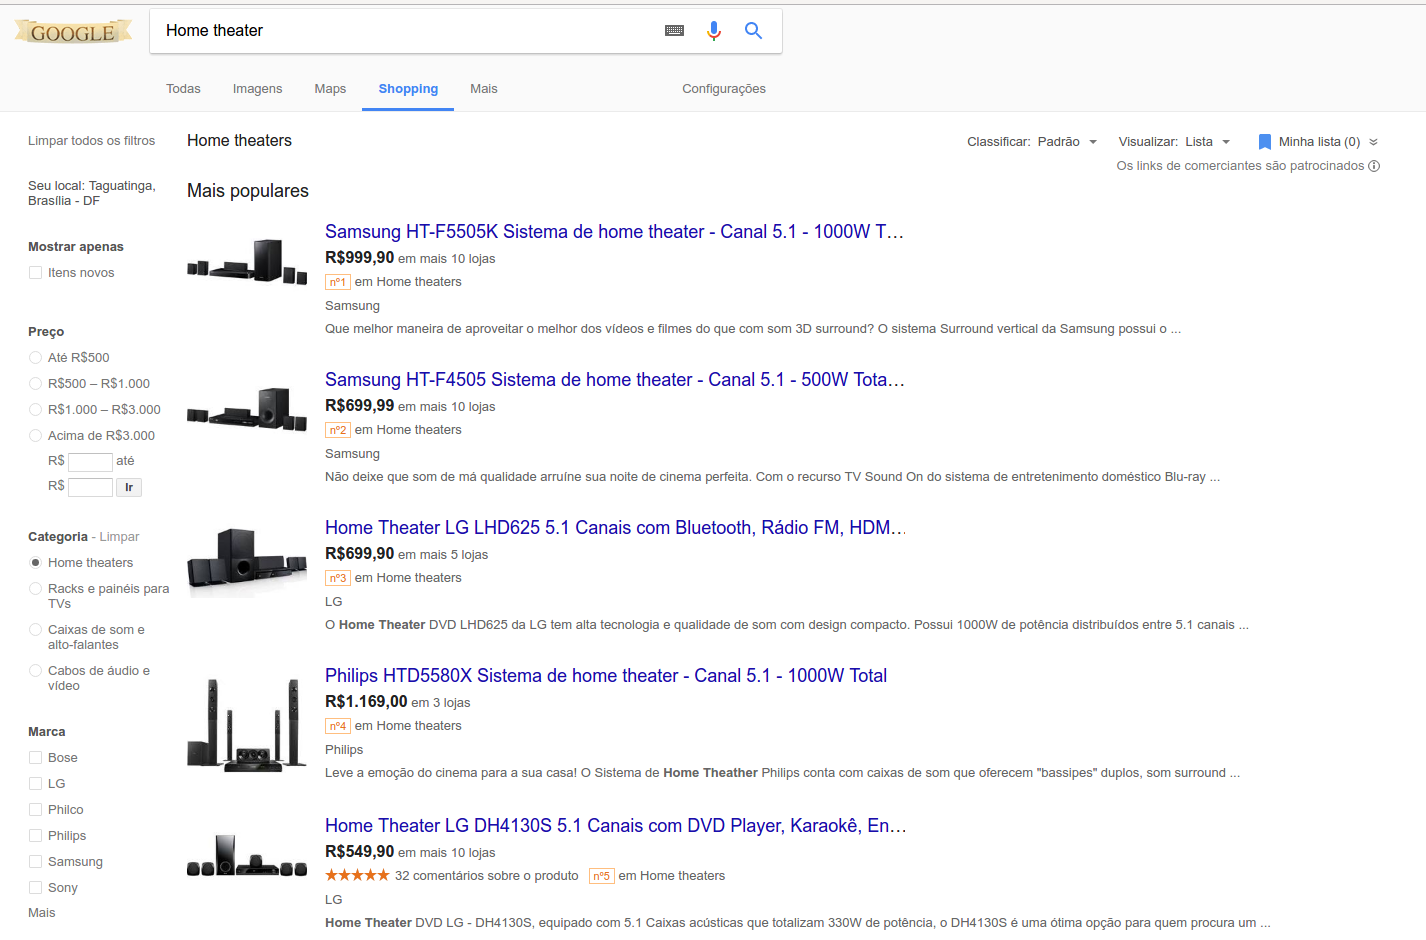
\includegraphics[keepaspectratio=true,scale=0.3]{figuras/GoogleBusca.png}
	\caption{Busca Google com SEO}
	\label{fig02}
\end{figure}

\section{Web Semântica e E-Commerce}

É a intersecção da tecnologia semântica e do \textit{E-Commerce}. Nesse tipo de negócio temos a busca de elementos tratadas e relacionadas semânticamente para direcionar um consumidor dentro de uma página a ofertas específicas baseadas no que eles está visualizando ou comprando. Esta tecnologia utiliza dados informados a partir de sites, redes sociais, opiniões de consumidores e a própria busca para aumentar a taxa de conversão.

Uma busca em uma plataforma que aplica Web Semântica como na figura \ref{fig03}:

\begin{figure}[h]
	\centering
	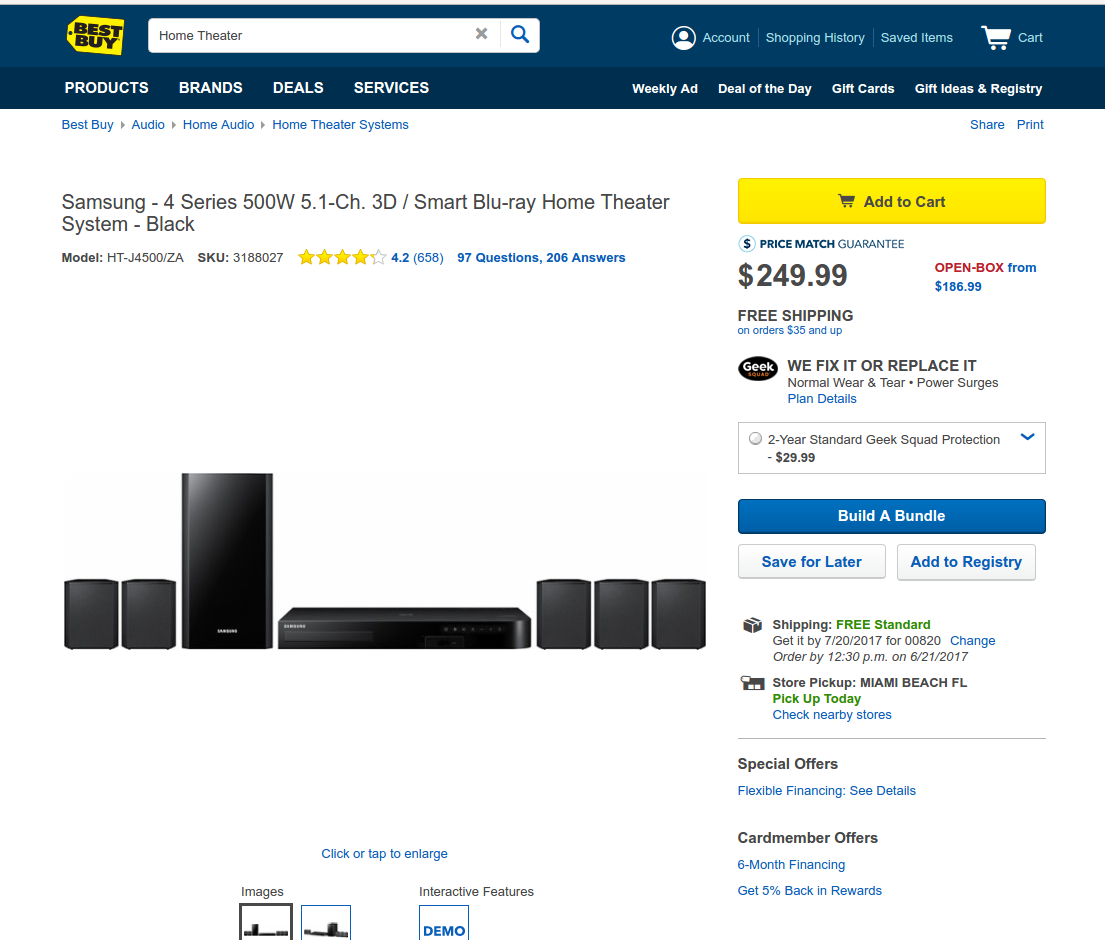
\includegraphics[keepaspectratio=true,scale=0.3]{figuras/HomeBusca.png}
	\caption{Busca Best Buy com Web Semântica}
	\label{fig03}
\end{figure}

Essas seriam as propostas de compra, relacionadas ao que se busca na figura \ref{fig04}:

\begin{figure}[h]
	\centering
	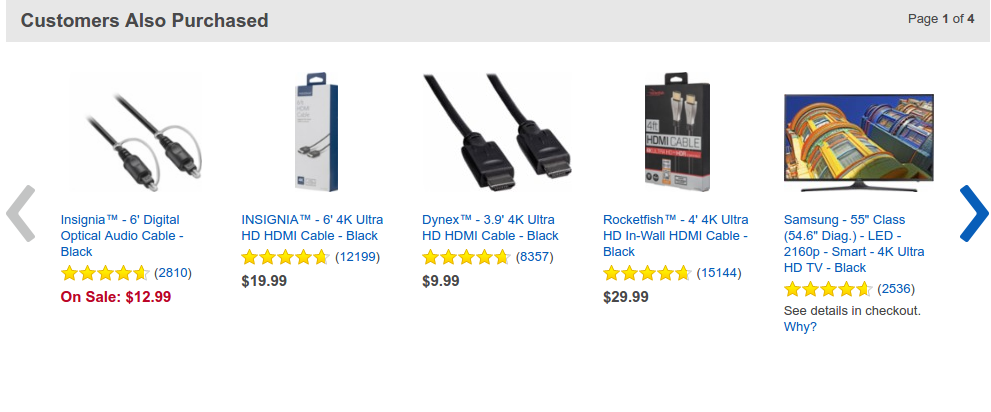
\includegraphics[keepaspectratio=true,scale=0.3]{figuras/HomeResultado.png}
	\caption{Propostas de compra com Web Semântica}
	\label{fig04}
\end{figure}


\chapter{Proposta de trabalho}

\section{Considerações iniciais}
	Neste capítulo vamos detalhar e introduzir a definição da proposta de trabalho, assim como o caráter da empresa, cronogramas e resultados esperados para quando o trabalho estiver concluído e as atividades que serão realizadas para que esse resultado seja alcançado
.
\section{Visão geral da proposta}
	O seguinte trabalho visa refinar o \textit{framework GoodRelations} de ontologia baseado em um contexto de uma empresa específica, para que possa ser usado de forma mais eficiente, voltada para o mercado brasileiro, visto que o \textit{framework} é de baixo nível, genérico e utilizado principalmente no mercado exterior, sendo pouco difundido no Brasil. Sabendo que a taxa de conversão pode ter um aumento considerável, como já mostrado neste trabalho e que pode gerar valor agregado ao cliente, será focado a ontologia a ser aplicada em uma empresa de distribuição e consultoria de produtos para restaurantes, bares e hotéis. 

\subsection{Atividades}
	Para chegar ao resultado esperado, vamos utilizar algumas técnicas, definidas anteriormente, para ter entendimento de quais são as necessidades do cliente e, principalmente, montar uma ontologia que esteja de acordo com seu modelo de negócio, para que possa ser de ajuda, na construção de um \textit{E-Commerce} com inteligência Web Semântica, serão estas as técnicas, já explicadas e embasadas anteriormente:

\begin{itemize}
	\item Acompanhamento de processo - Entender como o processo de venda é feita, acompanhando o cliente, para melhor compreender o ambiente e o processo.
	\item \textit{Brainstorm} - Conversa livre onde várias ideias são jogadas e analisadas posteriormente para formar aspectos que deverão ser apoiados pela ontologia.
	\item Entrevistas - Conversa direta com o cliente e interessados na solução.
	\item Protopitação - Modelos não funcionais de telas e exemplos de utilização das páginas a serem construídas.
	\item Questionário - Perguntas diretas que possam captar e entender melhor a visão do cliente, servem também como uma validação de requisitos.
\end{itemize}

\subsection{Estado da arte}
	A pesquisa não gerou muitos resultados a respeito de \textit{E-Commerce} aplicando \textit{Web Semântica} em território nacional, visto que não é amplamente divulgado e ainda pouco estudado, apesar seu seu crescimento constante. Temos parâmetros para analizar alguns casos fora do Brasil, como, por exemplo, a já citada, Best Buy, que utiliza  \textit{Web Semântica} para propor produtos a seus clientes, como uma comparação na tabela \ref{tab01}.
	\begin{table}[h]
		\centering
		\caption{Tabela de comparação Best Buy x Mercado Brasileiro}
		\label{tab01}
		\begin{tabular}{|l|l|}
			\hline
			Empresa            & 2016                     \\ \hline
			Best Buy           & 7.99 bilhões de Dólares  \\ \hline
			Mercado brasileiro & 20.33 bilhões de Dólares \\ \hline
		\end{tabular}
	\end{table}

Podemos notar grande diferença entre o mercado exterior comparado ao Brasil, principalmente, por que temos plataformas e \textit{Web Sites} defasados e sem preparo para \textit{Web Semântica}.
Como podemos ver na figura \ref{fig05}.

	\begin{figure}[h]
		\centering
		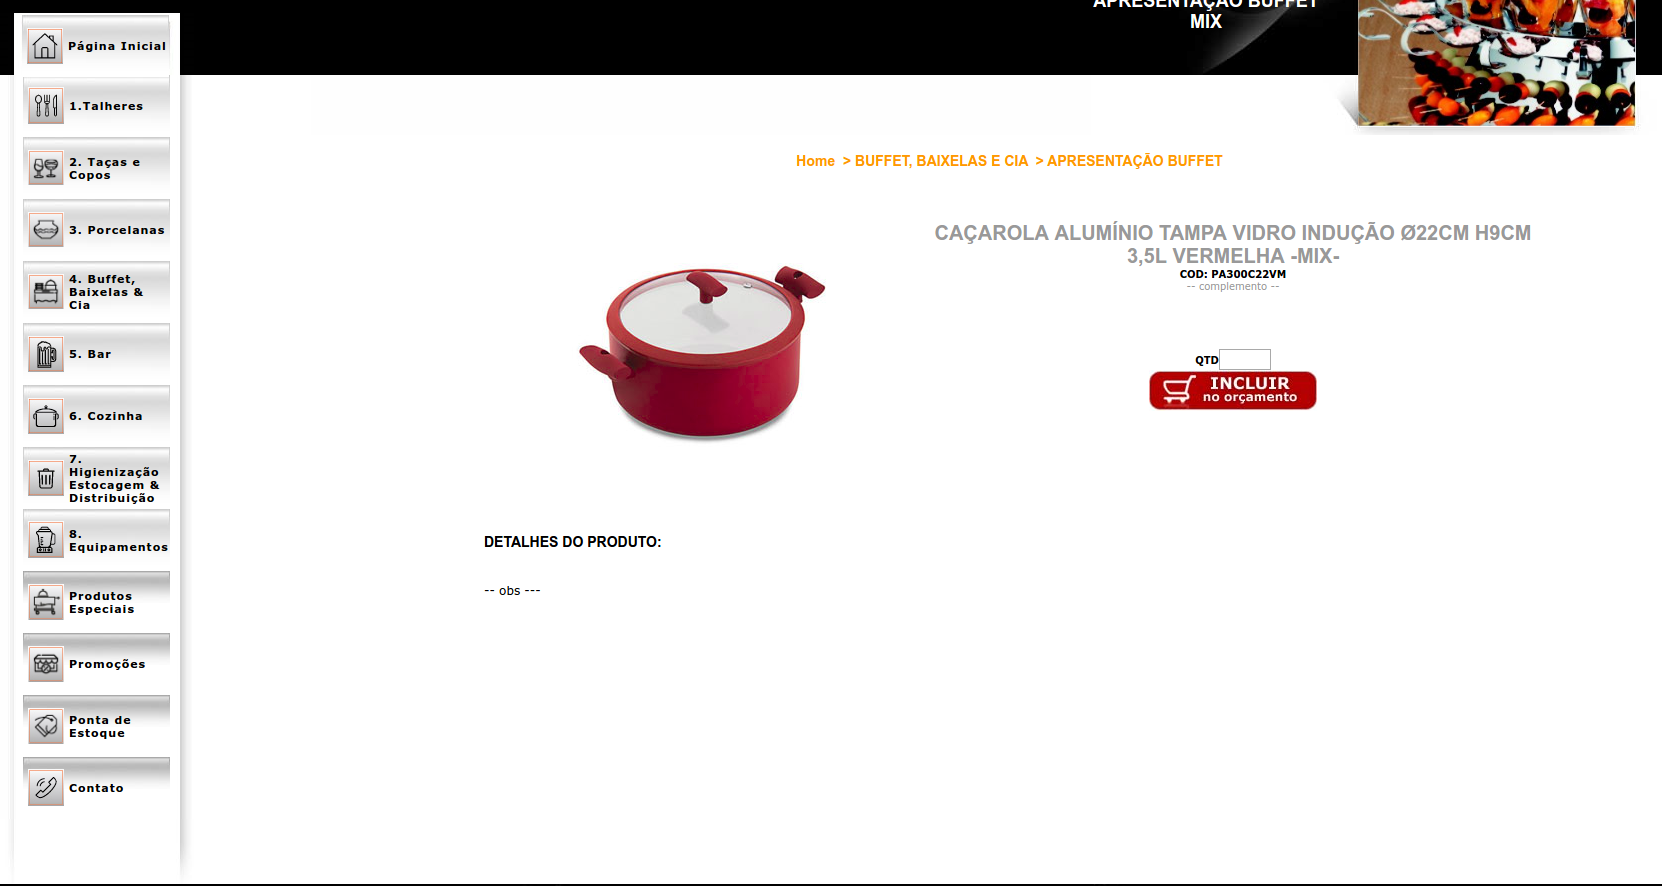
\includegraphics[keepaspectratio=true,scale=0.3]{figuras/SchipperProduto.png}
		\caption{Resultado de uma busca em um site de vendas de produtos de hotelaria}
		\label{fig05}
	\end{figure}

\section{Suporte tecnológico}

Seção que descreve ferramentas que serão usadas para desenvolver os artefatos para construção da solução proposta.

\subsection{Astah Professional}

Ferramenta de modelagem UML desenvolvida em Java, muito utilizada em modelagem de sistemas por sua variedade de diagramas, auxiliará no desenho da solução. O Astah\footnote{\url{http://astah.net}} é uma ferramenta que precisa ser liscenciada, portanto, será usada em seu período \textit{trial} de 30 dias.

\subsection{\textit{Protégé}}

Editor de ontologias desenvolvido pela \textit{University of Stanford}. Tem como objetivo a construção e manipulação de ontologias. O \textit{Protégé}\footnote{\url{http://protege.stanford.edu/}} é de livre acesso para fins educacionais, será utilizado para inserir e editar dados para criação de uma base de conhecimento.

\subsection{\textit{Spring Tool Suite}}

Ambiente que pornece uma IDE pronta para implementar, depurar e executar código Java, será usada para criação dos protótipos a serem mostrados para o cliente. O Spring\footnote{\url{http://spring.io/tools}} é de livre uso.

\section{Resultados Parciais}

A partir da pesquisa bibliográfica e uma pesquisa de mercado, podemos concluir que existe um grande espaço aberto a ser entendido quando falamos do relacionamento entre o comércio virtual e a \textit{Web Semântica} definimos uma metodologia, que aplicada, ajudará a entender melhor o problema e abrir caminhos para outros estudos e soluções que queiram atacar o mesmo nicho, que é o objetivo deste projeto.

Precisa-se entender o contexto a ser trabalhado para gerar a ontologia para este caso, desta forma, a aplicação das técnicas de elicitação de requisitos são necessárias para o avanço da criação da ontologia.

